\documentclass[11pt,a4paper]{article}

% ---------- Packages ----------
\usepackage[margin=0.75in]{geometry}
\usepackage[T1]{fontenc}
\usepackage{lmodern}
\usepackage{microtype}
\usepackage{graphicx}
\usepackage{booktabs}
\usepackage{tabularx}
\usepackage{longtable}
\usepackage{array}
\usepackage{enumitem}
\usepackage{xcolor}
\usepackage[hidelinks]{hyperref}
\usepackage{amsmath}
\usepackage{float}
\usepackage{caption}
\usepackage{pgfgantt}
\usepackage[numbers]{natbib}
\usepackage{natbib}
\definecolor{timelineblue}{HTML}{365B78}
\newlength{\timelineunit}
\setlength{\timelineunit}{\dimexpr(\textwidth-6.2cm)/10\relax}
\ganttset{
    hgrid={draw=gray!18},
    vgrid={*{3}{draw=gray!18},*{1}{draw=gray!45},
        *{3}{draw=gray!18},*{1}{draw=gray!45},*{1}{draw=gray!18}},
    x unit=\timelineunit,
    y unit title=0.55cm,
    y unit chart=0.72cm,
    title height=1,
    bar height=0.44,
    group height=0.35,
    milestone height=0.48,
    milestone left shift=0.2,
    milestone right shift=-0.2,
    bar label font=\footnotesize,
    group label font=\footnotesize\bfseries,
    milestone label font=\footnotesize\itshape,
    title label font=\scriptsize\bfseries,
    bar label node/.append style={text width=5.8cm, align=flush right},
    group label node/.append style={text width=5.8cm, align=flush right},
    milestone label node/.append style={text width=5.8cm, align=flush right},
    bar/.append style={fill=timelineblue!65, draw=timelineblue},
    group/.append style={fill=timelineblue, draw=timelineblue},
    milestone/.append style={fill=timelineblue, draw=timelineblue},
    title/.append style={fill=timelineblue!8, draw=gray!35},
    progress label text={}
}
\captionsetup{font=small, labelfont=bf, skip=6pt,
    justification=raggedright, singlelinecheck=false}
\captionsetup[table]{position=top}
\newcolumntype{Y}{>{\raggedright\arraybackslash}X}


% ---------- Hyperlink settings ----------
\hypersetup{
    colorlinks=true,
    linkcolor=blue,
    urlcolor=blue,
    citecolor=blue
}

% ---------- Custom commands ----------
\newcommand{\projecttitle}{\textbf{Reliable Multimodal Evaluation with Cascaded MLLM Judges}}
\newcommand{\course}{CS 613: Natural Language Processing}
\newcommand{\semester}{Sem-I, 2026--27}
\newcommand{\repo}{\url{https://github.com/TODO/your-repository}}
\newcommand{\datasetlink}{\url{TODO}}
\newcommand{\paperlink}{\url{TODO}}

\setlength{\parindent}{0pt}
\setlength{\parskip}{4pt plus 1pt}
\setlength{\intextsep}{9pt plus 2pt minus 2pt}
\setlength{\tabcolsep}{7pt}
\renewcommand{\arraystretch}{1.15}
\clubpenalty=10000
\widowpenalty=10000
\setlist[itemize]{noitemsep, topsep=3pt}
\setlist[enumerate]{itemsep=2pt, parsep=0pt, topsep=4pt}

\begin{document}

% ---------- Title page ----------
\begin{titlepage}
    \centering
    
    {\Large \textbf{Indian Institute of Technology Gandhinagar}\par}
    \vspace{0.25cm}
    {\large \course \par}
    {\large \semester \par}
    
    \vspace{1.4cm}
    \rule{\textwidth}{0.6pt}
    
    \vspace{0.6cm}
    {\LARGE \textbf{ASSIGNMENT 1 REPORT}\par}
    \vspace{0.45cm}
    {\Large \projecttitle\par}
    
    \vspace{0.6cm}
    \rule{\textwidth}{0.6pt}
    
    \vfill
    
    \begin{tabular}{rl}
        \textbf{Lead TA:} & Naren Kumar \\
        \textbf{Repository:} & \url{https://github.com/ShardulJunagade/cascaded-selective-evaluation} \\
        \textbf{Submission Date:} & September 06, 2026 \\
    \end{tabular}
    
    \vspace{1cm}
    
    \begin{table}[H]
    \centering
    \begin{tabularx}{0.9\textwidth}{|X|X|X|}
        \hline
        \textbf{Name} & \textbf{Roll Number} & \textbf{Email} \\
        \hline
        Patel Ridham Vijaykumar & 23110238 & ridham.patel@iitgn.ac.in \\
        \hline
        Anurag Singh & 23110035 & singh.anurag@iitgn.ac.in \\
        \hline
        Arjun B. Dikshit & 23110040 & 23110040@iitgn.ac.in \\
        \hline
        Abhinav Khot & 23110006 & abhinav.khot@iitgn.ac.in \\
        \hline
        Parth Dembla & 23110234 & parth.dembla@iitgn.ac.in \\
        \hline
        Shardul Junagade & 23110297 & shardul.junagade@iitgn.ac.in \\
        \hline
        Shriniket Behera & 23110306 
& shriniket.behera@iitgn.ac.in \\
        \hline
        Rathod Yuvraj Rajubhai & 24110293 & yuvraj.rathod@iitgn.ac.in \\
        \hline

    \end{tabularx}
    \end{table}
    
    \vfill
    
    {\small
    We affirm that this report and its accompanying code have been prepared in
    accordance with the IIT Gandhinagar Honor Code. \\
    \textbf{AI Usage Disclosure}: The latex template was generated using ChatGPT 5.5. The content is ideated and written by the team, with AI used only for grammatical corrections in some places. Existing work is duely cited, and team members are fully responsible for the written text.
    \par}
\end{titlepage}

\tableofcontents
\newpage

% ============================================================

\section{Introduction}

\subsection{Motivation}

Automatic evaluation is becoming essential as modern language and vision-language systems produce far more outputs than humans can manually judge. However, LLMs are not always reliable judges of response quality. Prior work has flagged concerns regarding validity and reliability of usage of LLM-based evaluators as an alternative to human judgment, especially when their decisions are treated as authoritative without careful calibration~\cite{chehbouni2025neither}. This is where the scope of methods that gives control in the hands of human user, with a guaranteed reliability of the model as a judge.
There have been attempts to solve this issue in context of text-only LLMs in the paper, \textit{Trust or Escalate}. They addresses this issue for LLM judges by using cascaded selective evaluation, where a judge only answers when its confidence passes a calibrated threshold and otherwise escalates the example to a stronger evaluator~\cite{jung2025trust}. However, this framework was only framed for text-only LLM evaluation. Such solutions are yet to exist for multi-modal LLMs. Therefore, in our project, we aim to extend the above mentioned paper's risk-controlled idea to multimodal systems, where responses may depend on image context and even audio context. Solving this problem is important and non-trivial because VLMs introduce additional sources of error, such as visual hallucination and modality bias~\cite{zheng2025modality}. Our goal is therefore to bridge the gap between expensive human evaluation, unreliable uncalibrated model judges, and the growing need for trustworthy evaluation of multimodal outputs. 

The risk of failure of the project is minimal as per initial judgement \& experiments in this assignment, although, this project posseses the risks of failure while scaling it. As the mathematical work already exist in single modality, extending it to multiple ones become a feasible research problem, and a mathematically grounded framework has a greater probability of experimental success. 
% In those scenarios, the exploration of statistically reliable multimodal judges will remain underdeveloped.

\subsection{Relation with NLP}

This is still an NLP problem because the main goal is to evaluate natural-language responses, their confidence, and which response is preferred. Even techniques used for interpretation of visual and audio inputs in the current MLLM models draw inspiration from textual NLP and extend them \cite{YAO2026116569}. In this sense, the project extends traditional NLP evaluation from text-only settings to multimodal settings, where models must combine visual evidence with natural language understanding.

% This project remains an NLP problem because the central object being evaluated is a natural-language response combined with probabilistic confidence modeling, and the final decision is a language-mediated preference judgment. Even when the input includes an image, the judge must interpret a natural language instruction, compare two textual answers, and decide which response better satisfies the human preference. The image acts as context, but the reasoning, comparison, confidence estimation, and final output are all expressed through NLP methods. In this sense, the project extends traditional NLP evaluation from text-only settings to multimodal settings, where models must combine visual evidence with natural language understanding.

\subsection{Problem Type}

This project is mainly about the problem of judging which response is better, with an added focus on making that judgment reliable. For each example, the system sees some multimodal context, an instruction, and two possible responses, then chooses whether response A or response B is preferred. This makes it closer to a classification problem than a text-generation problem, because the final answer is a fixed choice rather than a newly written response. 
% We also use a few examples of human preferences in the prompt, so the judge can follow the style of human annotation without being retrained. 
The key difference from a normal classifier is that our system does not have to answer every time: if it is not confident enough, it can abstain or pass the example to a stronger judge. By calibrating this confidence threshold, we provide a theoretically backed way to accept only those model judgments that are likely to agree with human preferences.

% The problem is best identified as nested selective classification with confidence calibration for reliable results. For each example, the evaluator receives a context, an instruction, and two candidate responses, then predicts a discrete preference, indicating whether response A or response B is better. The judges are prompted with few-shot examples of human preferences, which act as simulated annotator demonstrations. Unlike ordinary classification, the evaluator is allowed to abstain when its confidence is below a calibrated threshold. In the cascaded setting, easier examples are handled by smaller judges, while uncertain examples are escalated to stronger models. The main task is therefore not supervised training, but few-shot preference classification combined with calibration of confidence thresholds so that accepted judgments agree with human preferences at the desired reliability level.
% ============================================================
\section{Related Work}

\subsection{State of the Art}

The main State of the Art paper that solves the problem for evaluation tasks with LLM Judges (with theoretical guarantees) for purely text based tasks is \emph{Trust or Escalate: LLM Judges with Provable Guarantees for Human Agreement} by Jung et. al \cite{jung2025trust}. For this entire section we derive facts and results from this paper. This paper produces a method that provides the following theoretical guarantee

$$
P(f_{LM}(x) = y_{human}|c_{LM}(x) \geq \lambda) \geq 1 - \alpha
$$

holds with probability $1 - \delta$ for a user defined tolerances $\alpha$ and $\delta$. Here $f_{LM}$ is the judgement given by the LLM judge and $y_{human}$ is the human's judgement. $c_{LM}(x)$ is the confidence of the judge for the evaluation instance $x$.  It basically says that given that the confidence of the judge LLM is above a calibrated threshold $\lambda$, the evaluation result it gives agrees with human evaluation for the same instance $1-\alpha$ fraction of times, with a probability 1 - $\delta$.

The main method that the authors propose is \textbf{Cascaded Selective Evaluation}. This method can be very easily understood using Fig \ref{fig:cse}

\begin{figure}[H]
    \centering
    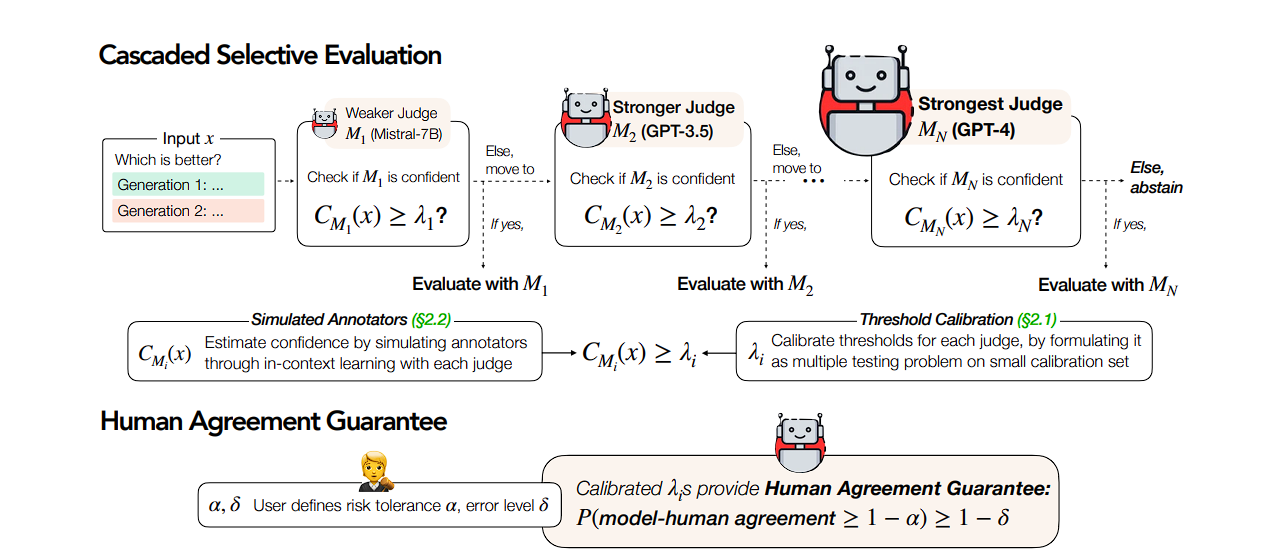
\includegraphics[width=1\linewidth]{CASCADESELECTIVE.png}
        \caption{Cascaded Selective Evaluation}
    \label{fig:cse}
\end{figure}

The key idea is that we have a chain of models and at each stage the LLM judge outputs a result with a confidence value. If this confidence is above the threshold for that stage, we accept the judgement, else we pass it on to the next model in the chain. The confidence is estimated by using \emph{Simulated Annotators}, a concept the authors introduce. The basic idea is that we created $r$ personas of the same judge by giving it different $K$ examples along with the evaluation prompt (essential each \emph{Simulated Annotator} is a K-shot prompt to the LLM judge) and the confidence is the fraction of the judges agreeing with the majority result.

The values of the thresholds $\lambda_i$ at each stage of the chain are calibrated using a hold out small calibration set.

This paper is novel since it introduces these guarantees and also the framework proposed outperforms individual high parameter models by themselves (for e.g it achieves over 80\% human agreement on the ChatArena dataset while covering over 79\% of all test cases). This framework also leads to significant cost savings since a lot of the times the lower cheaper models in the chain produce a confident result before escalating to the more expensive models (In the earlier mentioned result, over 88\% of evaluated tests were done before reaching the final model in the chain).
\subsection{Available Baselines and Implementations}

The authors provide the implementation of the proposed framework as part of a \href{https://github.com/jaehunjung1/cascaded-selective-evaluation}{GitHub} Repository in the paper itself.

The authors also provide baseline comparisons with other confidence estimation methods. For e.g they compare methods like: Asking the LLM Judge itself to report confidence values, Predictive Probability, Randomized Annotators etc. and show that the proposed \emph{Simulated Annotators} is the best method among these which does not over confidently predict LLM Judgements (and thus this would maximize test coverage too). 

The authors also provide baseline comparisions with just using GPT-4 as a single judge instead of the proposed framework. They evaluate metrics like Empirical Human Agreement, Coverage and Guaranteed Success rate (The fraction of times the empirical human agreement is above the threshold $1 - \alpha$ we set, over a large set of runs).
\subsection{Previously Reported Results}

The paper reports a large amount of result data, and we have summarized a few important ones below (These are taken verbatim as images from the paper). 

\begin{figure}[H]
    \centering
    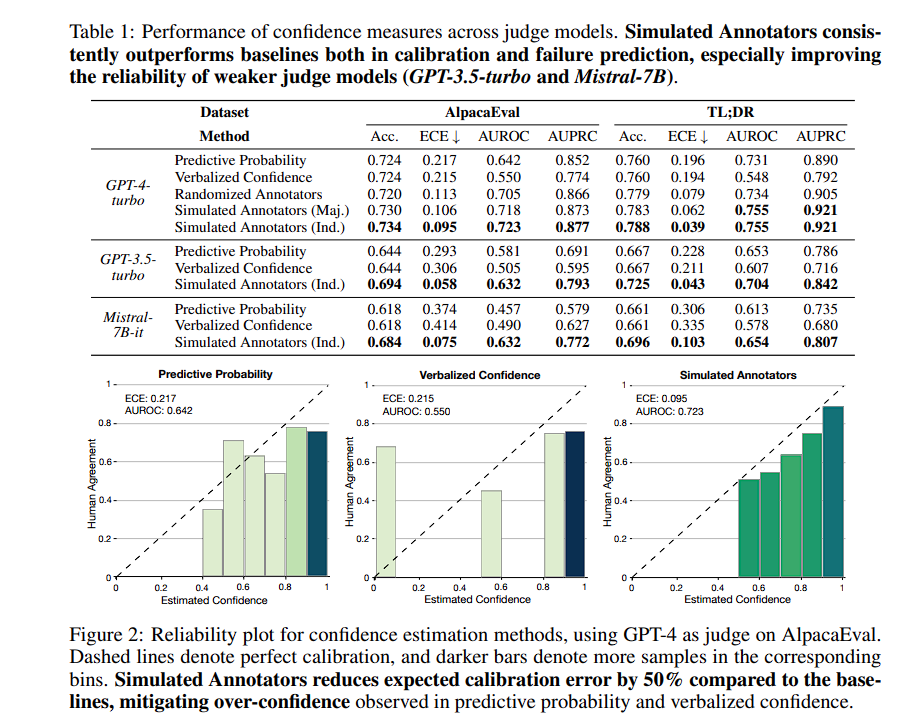
\includegraphics[width=1\linewidth]{simulanot.png}
    \caption{Reported results for simulated annotators from the original paper.}
    \label{fig:simulanot}
\end{figure}

\begin{figure}[H]
    \centering
    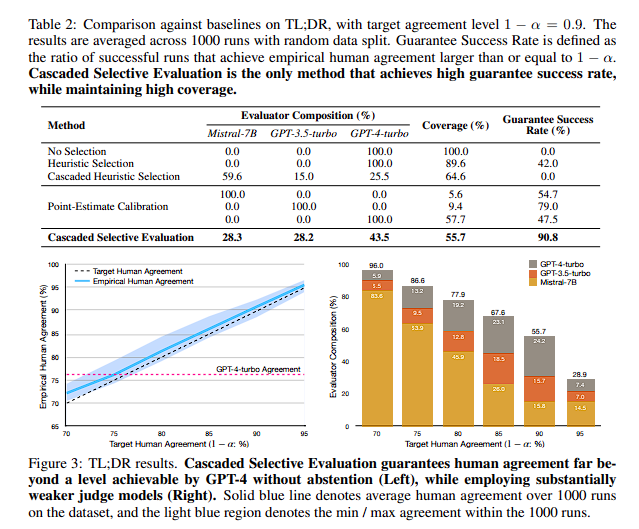
\includegraphics[width=1\linewidth]{summres.png}
    \caption{Summary of results reported in the original paper.}
    \label{fig:reported-results}
\end{figure}

\begin{figure}[H]
    \centering
    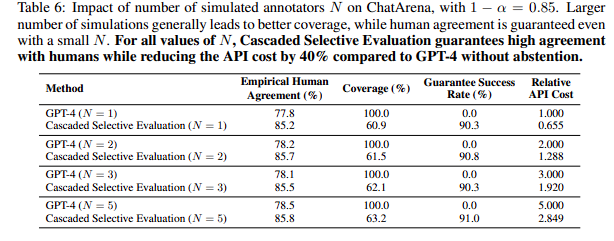
\includegraphics[width=1\linewidth]{gptvsours.png}
    \caption{Reported comparison of cascaded selective evaluation with a single GPT-4 judge.}
    \label{fig:gpt4-comparison}
\end{figure}




\section{Datasets}

The datasets used in \citet{jung2025trust} are TL;DR \citep{stiennon2020learning} for
summarization, and ChatArena \citep{li2024dissecting} and Auto-J \citep{li2023generative}
for chat assistant evaluation. Each instance in these has a query, two model responses and
a human preference label saying which response is better.

We need the same structure with an image added. Every instance should have

\begin{itemize}
\item an image and a prompt,
\item two responses generated by two different VLMs, and
\item a human preference label choosing one of the two.
\end{itemize}

The label has to be a forced choice between the two candidates, because the calibration
step needs every instance to behave as a pass or fail trial. Two more properties which are required in the data are:

\begin{itemize}
\item \textbf{Annotator ids.} Simulated Annotators needs $K$ preference examples
drawn from each of $N$ individual annotators, so the labels must be attributable to
specific annotators.
\item \textbf{Repeated annotation.} The abstention analysis needs more than one annotation
on the same instance, so that inter annotator agreement (IAA) can be computed.
\end{itemize}

Table \ref{tab:datasets} lists the
candidates we identified, and we draw on them as required depending on which properties a
given experiment needs.

\begin{table}[h]
\centering
\small
\begin{tabular}{lllll}
\toprule
\textbf{Dataset} & \textbf{Task domain} & \textbf{Size} & \textbf{Label type} & \textbf{Annotator info} \\
\midrule
VisionArena-Battle & In the wild chat & 30K convs & Forced choice & User id, 1 vote \\
VisIT-Bench & Instruction following & 5K judgments & Forced choice & 5 per tuple \\
JudgeAnything & 15 any to any tasks & 3,000 pairs & Forced choice & 12 annotators, 15 per item \\
MM-RLHF & General, image and video & 16,342 prompts & Ranking & No id field \\
RLHF-V & Hallucination & 1.4K instances & Correctional edit & No id field \\
\bottomrule
\end{tabular}
\caption{Candidate datasets for multimodal selective evaluation.}
\label{tab:datasets}
\end{table}

\textbf{VisionArena-Battle} \citep{chou2024visionarena} contains 30K conversations
collected from an online arena, where users uploaded an image, asked their own question,
and voted between responses from two anonymous VLMs drawn from a pool of 19. It spans
roughly 23K unique images and 90 languages. Each row holds the two model names, the two
conversations, a winner label with the values model\_a, model\_b, tie and tie (bothbad), a
\texttt{judge} field holding a hash of the voting user, and category tags such as
captioning, OCR and diagrams.\footnote{\url{https://huggingface.co/datasets/lmarena-ai/VisionArena-Battle}}

\textbf{VisIT-Bench} \citep{bitton2023visit} contains 679 instances and 1,578 images across
70 instruction families, with responses from seven models and a human verified GPT-4
reference. It provides 5K pairwise human judgments, collected as 5 crowdworker judgments
each on 1K sampled tuples of query, model A and model B, in a forced choice setting with no
tie option.\footnote{\url{https://github.com/mlfoundations/VisIT-Bench}}

\textbf{JudgeAnything} \citep{pu2025judgeanything} covers 15 any to any modality
combinations built on 1,500 queries spanning text, image, video and audio, with four models
generating responses per query. It provides 3,000 pair comparison instances, each with a
task specific checklist, annotated by 12 annotators with cross-validation
between annotators, giving 15 annotations per item and 45,000 human judgments in
total.\footnote{\url{https://urrealhero.github.io/judgeanythingweb/}}

\textbf{MM-RLHF} \citep{zhang2025mmrlhf} contains 16,342 prompt-level instances covering
image, video and safety content. More than 50 expert annotators scored each candidate
output on faithfulness, helpfulness and ethical dimensions, and produced a final ranking
over the outputs together with a written rationale.\footnote{\url{https://huggingface.co/datasets/yifanzhang114/MM-RLHF}}

\textbf{RLHF-V} \citep{yu2024rlhfv} contains 1.4K instances of fine-grained correctional
human feedback. Each instance holds an image, a prompt, a model response, and a human
edited version of that response in which the hallucinated segments have been
corrected.\footnote{\url{https://github.com/RLHF-V/RLHF-V}}

\subsection{Dataset curation pipeline}

All five datasets are publicly available and already carry human preference labels, so no
crawling and no additional annotation is required. The labels are not balanced, and
the skew is different in each one. RLHF-V is the most skewed of the five, because the preferred side is
always the human corrected response. This is why we treat it as a pilot rather than a main result,
as described in Section 6. VisIT-Bench leans in a similar direction as, the strongest model wins against the human verified reference in only $27.4\%$ of
comparisons. The remaining two are skewed in ways that depend on how we
process them rather than on how they were collected. VisionArena carries four label values
instead of two, so the two tie classes have their own frequencies and removing them shifts
the balance of what is left. MM-RLHF has no fixed distribution at all, since its pairs are
derived from rankings and the score gap threshold we pick decides how easy the resulting
comparisons are. We therefore report the label counts for each dataset after filtering, and
apply the steps below to bring the five sources into a common format.

\begin{enumerate}
\item \textbf{Filtering.} Keep only the instances that the judge prompt can accept. The
input must be a single image (or some other modality) together with a text prompt, and both responses being compared must be text. Instances whose expected output is generated media, such as an image or an
audio clip, are removed, since there is nothing for a text judge to compare.
\item \textbf{Pair construction.} Datasets that already provide a forced choice between
two responses are used unchanged. On the other hand, datasets that provide ratings or a ranking over several
responses are converted into pairs, retaining only those pairs whose score gap exceeds a
threshold, so that near equal responses are not treated as clear preferences.
\item \textbf{Tie handling.} Tied instances are excluded from the main protocol, since a
forced choice risk is undefined when the annotator is indifferent. They are retained as a
separate set, which allows us to test whether the estimated confidence approaches its lower
bound of 0.5 where human preference is least determinate.
\item \textbf{Position randomization.} The assignment of the two responses to positions A
and B is randomized, to control for the position bias reported for judge models
\citep{wang2023large}.
\item \textbf{Overlap removal.} Sources are checked for shared queries before being
combined, since several of these benchmarks sample from one another, and duplicated
instances are removed from one side.
\item \textbf{Annotation grouping.} This step depends on what a dataset provides. If an
instance carries more than one annotation, we aggregate them into a majority label and an
agreement level, which is what the abstention analysis compares against. If the labels
carry annotator identifiers, we group them by annotator to build the in context pools for
Simulated Annotators (Ind.). An annotator needs at least $K+1$ labels to be usable here,
since $K$ of them go into the prompt as few shot examples and at least one must be left
out for evaluation, so annotators below this count are dropped.
\item \textbf{Splitting.} Each dataset is partitioned into a calibration set and a test
set, with a reduced calibration size for the smaller benchmarks.
\end{enumerate}





% ============================================================
\section{Experimental Plan}

We port \emph{Trust or Escalate: LLM Judges with Provable Guarantees for Human Agreement}
\citet{jung2025trust} from text only LLM
judges to vision-language model (VLM) judges. A cascade of VLM judges evaluates
pairs of image-grounded responses (captions, VQA answers, or multimodal chat responses). We calibrate an confidence threshold ($\lambda$) per judge so that, when we receive a result from any model on the cascade (i.e when the entire cascade of models does not abstain)  we can guarantee (with high probability $1-\delta$ ) that its preference agrees with human judgment at a user-specified level $1-\alpha$.
 
\subsection{Experimental Setting}
 
\subsubsection{Dataset Split}

The method has no trainable parameters, so no conventional train split is required. However, we split the dataset into the calibration set $D_{cal}$ and the test set $D_{test}$:
 
\begin{itemize}[leftmargin=*]
    
  \item We construct instances
        $(\text{image}, \text{query}, a_1, a_2, y_{human})$ from the chosen  where $a_1$ and $a_2$ are the generated responses and $y_{human}$ is the annotator preferences.
  \item Set the $\delta$ value for the experiment.
  \item We run the calibration and evaluation procedures over many random splits of the chosen
        dataset into $D_{cal}$ and $D_{test}$ and we report results averaged across all runs. This is necessary because a
        single split does not empirically establish whether the probabilistic guarantee (1-$\delta$)  holds.
  \item A small portion of the chosen dataset is reserved as a development subset to select $K$ (number of in-context
        examples per simulated annotator) and $N$ (number of simulated annotators) for the cascade, before any calibration or testing is performed. This subset is never
        reused as $D_{cal}$ or $D_{test}$.
\end{itemize}
 
 
\subsubsection{Finding Best Parameters for Algorithms and Baselines}
 
We select our hyperparameters in the following methods:
 
\begin{itemize}[leftmargin=*]
  \item  $N$ is determined by the number of
        annotator-specific few-shot sets prepared, and $K$ is the
        number of in-context examples drawn per annotator from that set. Unlike the original
        paper, which uses $K \le 5$, our VLM prompts embed an image per few-shot example, so context length constrains $K$ to a much smaller range in practice. Accordingly, the dev-subset sweep is restricted to a smaller grid
        (e.g.\ $K \in \{1,2\}$, $N \in \{1,2,3,5\}$) and determined by evaluating ECE, AUROC, and
        AUPRC of the confidence measure for each judge.
\item For each judge, confidence per simulated annotator is
        computed from the model's label-token logprobs on the preference tokens (predictive probability over labels, per annotator prompt), then aggregated across the $N$ simulated
        annotators following the Simulated Annotators formulation.
  \item For each judge model $M_i$ in the cascade, $\lambda_i$ is analytically derived for each calibration split using fixed sequence testing, rather than being selected through grid search. We first calculate the empirical disagreement risk $\widehat{R}(\lambda)$ at every candidate threshold on $D_{cal}$, which is defined as the fraction of instances on which the judge disagrees with the human label among the instances that it would evaluate at that threshold. Because this risk is estimated from a finite sample, we subsequently compute its exact $(1-\delta)$ upper confidence bound $\widehat{R}^{+}(\lambda)$, which accounts for sampling variability and ensures that the true risk is not underestimated. We then select the smallest threshold for which this upper bound remains below the target risk $\alpha$:

\[
        \widehat{\lambda}_i = \inf\left\{\lambda : \widehat{R}^{+}(\lambda') \le \alpha \ \ \forall \lambda' \ge \lambda\right\}.
      \]

This procedure is applied sequentially down the cascade: $\lambda_i$ is calibrated only on the subset of $D_{cal}$ on which judges $M_1,\ldots,M_{i-1}$ abstain, with an error budget of $\delta/|\mathcal{M}|$ assigned to each judge, ensuring that the guarantee holds jointly across the entire cascade rather than separately for each judge. 
  \item Baselines to reproduce with VLM judges:
        \begin{enumerate}[leftmargin=*]
  \item No Selection: always use \texttt{qwen2.5-vl-7b-instruct} (the strongest
        available judge in the cascade) to evaluate every instance, with no abstention.
  \item Heuristic Selection: use \texttt{qwen2.5-vl-7b-instruct} alone with
        $\lambda = 1-\alpha$, assuming the confidence measure is already perfectly calibrated.
  \item Cascaded Heuristic Selection: the same two judge cascade, but with
        $\lambda = 1-\alpha$ set heuristically at each stage instead of via fixed sequence
        testing.
  \item Point-Estimate Calibration: set $\lambda$ to the smallest value satisfying
        $\widehat{R}(\lambda) < \alpha$ on $D_{cal}$, without the finite-sample correction
        (i.e., without computing $\widehat{R}^{+}(\lambda)$).
  \item Cascaded Selective Evaluation: We employ the full methodology. We perform fixed sequence testing
        applied sequentially per judge in the cascade, with error budget $\delta/|\mathcal{M}|$
        allocated across judges.
\end{enumerate}
\end{itemize}
 
\subsection{Metric}
 
Because the contribution will be a statistical guarantee, accuracy alone is insufficient. We
report the same metrics as the original paper, each capturing a distinct failure mode:
 
\begin{enumerate}[leftmargin=*]
  \item Empirical human agreement on non-abstained instances.
  \item Coverage: The percentage of instances not abstained on by the entire cascade (a method that abstains on
        everything trivially satisfies the guarantee but is useless).
  \item Guarantee Success Rate:  the fraction
      of runs achieving empirical agreement $\ge 1-\alpha$ across many random calibration/test splits. This empirically validates that the
      guarantee holds at least $(1-\delta)\times 100\%$ of the time, as predicted by the
      theoretical bound.
  \item ECE, AUROC, AUPRC of the confidence measure alone (pre-selection), to check
        whether Simulated Annotators transfers to VLMs as well as it does for text LLMs.
  \item Relative cost (API calls / compute, weighted by model size or price):  For understanding if cost is reduced while preserving
        guarantee after cascading.
\end{enumerate}


Furthermore, we perform experiments to analyze the effect of multimodality on the probabilistic
guarantees and accuracy of the cascading model. This includes ablations over the number of
simulated annotators $N$ and few-shot examples $K$ and comparing image-conditioned versus text-only confidence estimation to
isolate the contribution of visual grounding. We additionally analyze failure cases where
abstention correlates with visual ambiguity to test whether the confidence measure's
reliability generalizes from text-only to multimodal judgment. We also examine multimodal-specific biases (e.g.\ sensitivity to image resolution, object
position, or superficial visual features rather than content) through ablations that vary these
factors, testing whether the confidence measure remains reliable or systematically miscalibrates
under such shifts.


\subsection{System Effort and Demo Scenario}

The deliverable is a reproducible evaluation pipeline which includes a scoring pipeline for the VLM cascade, downstream scripts for cascade calibration and
evaluation across many random $D_{cal}$/$D_{test}$ splits, and a final results notebook/report
producing agreement vs $\alpha$ plots, a judge composition breakdown, results table of coverage and guarantee success rate.
 
\section{Project Management}

\subsection{Timeline}

The project is planned from September to the second week of November 2026.
Since the project is carried out alongside other CS~613 coursework, the
timeline focuses on the major research phases and prioritizes the core
reproduction and VLM experiments before final analysis and reporting.

\begin{figure}[H]
\centering
\begin{ganttchart}{1}{10}

\gantttitle{\shortstack{September\\2026}}{4}
\gantttitle{\shortstack{October\\2026}}{4}
\gantttitle{\shortstack{November\\2026}}{2} \\

\gantttitlelist{1,...,10}{1} \\

\ganttbar{1. Paper study \& project setup}{1}{2} \\

\ganttbar{2. Baseline reproduction}{2}{3} \\
\ganttbar{3. Dataset preparation \& VLM pipeline}{2}{3} \\

\ganttmilestone{Baseline ready}{3} \\

\ganttbar{4. Selective evaluation \& VLM extension}{4}{6} \\

\ganttbar{5. Cascade experiments \& statistical validation}{5}{8} \\
\ganttbar{6. Extension of Mathematical Analysis to VLMs}{7}{8} \\
\ganttmilestone{7. Main experiments with theoretical guarantees complete}{8} \\

\ganttbar{8. Final analysis, report \& presentation}{9}{10} \\
\ganttmilestone{9. Final submission}{10}

\end{ganttchart}
\caption{Planned project timeline from September to the second week of
November 2026.}
\label{fig:gantt}
\end{figure}

The project progresses from understanding and reproducing the original
framework to establishing the VLM pipeline, followed by selective
evaluation and cascade experiments. The final weeks are reserved for
statistical validation, analysis (experimental \& mathematical), documentation, and presentation.
Advanced experiments will be prioritized based on the available time and
computational resources.

\subsection{Computational Resources}

The experiments for this assignment are performed using open-weight VLMs on the NCAS delta computing environment (UIUC's HPC, that we have access to). For our initial replication, we use Qwen2.5-VL-3B-Instruct followed by Qwen2.5-VL-7B-Instruct, with vLLM for inference. We chose these instead of the exact models used in the paper, because the original paper uses some closed-source models such as GPT-3.5-turbo and GPT-4-turbo, whose model versions and API availability have changed over time. Using open-weight models allows us to run the models locally and have better control over the model and inference settings. The 72B VLM was not included in the initial cascade due to the available GPU budget.

% \begin{table}[H]
% \centering
% \small
% \caption{Computational resources required for the project.}
% \begin{tabularx}{\textwidth}{@{}>{\raggedright\arraybackslash}p{0.15\textwidth}Y@{}}
% \toprule
% \textbf{Resource} & \textbf{Requirement and purpose} \\
% \midrule
% GPU &
% Insert the actual NCSA Delta GPU allocation. GPUs are primarily
% required for inference with the Qwen2.5-VL-3B and Qwen2.5-VL-7B judges. \\

% CPU cores &
% Insert actual allocation. CPUs are required for dataset preparation,
% image processing, file management, and coordinating inference jobs. \\

% RAM &
% Insert actual allocation. System memory is required for loading
% multimodal data, image preprocessing, and inference orchestration. \\

% Storage &
% Insert actual allocation. Storage is required for datasets, image
% files, model/cache files, cached judge outputs, and experiment results. \\

% Software &
% Python, PyTorch, vLLM, Hugging Face libraries, and the existing
% Cascaded Selective Evaluation repository. \\

% \bottomrule
% \end{tabularx}
% \end{table}

\begin{table}[H]
\centering
\small
\caption{Computational resources required for the project.}
\begin{tabularx}{\textwidth}{@{}>{\raggedright\arraybackslash}p{0.15\textwidth}Y@{}}
\toprule
\textbf{Resource} & \textbf{Requirement and purpose} \\
\midrule

GPU &
1$\times$ NVIDIA A100-SXM4 GPU with 40\,GB HBM2 memory should be enough for accelerated
inference with the small Qwen-based judges. Larger models like 72B parametered Qwen may require multiple
GPUs or model parallelism depending on their memory requirements upto 144 GB. \\

CPU cores &
16 CPU cores per job. CPUs are used for dataset preparation,
image preprocessing, file I/O, and coordinating GPU inference. \\

RAM &
64\,GB of system memory per job. This is sufficient for dataset loading,
multimodal preprocessing, inference orchestration, and intermediate
results while the model computation is primarily performed on the GPU. \\

Storage &
Approximately 50\,GB of project and scratch storage for large pretrained model weights, source datasets,
processed images, model/cache files, cached judge outputs, logs, and
experimental results. \\

Software &
Python 3.12, PyTorch with CUDA support, Hugging Face Transformers and
Hugging Face Hub, vLLM where applicable, and the existing Cascaded
Selective Evaluation repository. \\

\bottomrule
\end{tabularx}
\end{table}

The use of a cascade also reduces computational requirements compared with
using the largest available VLM for every instance. The smaller VLM can
resolve sufficiently confident cases, while only uncertain cases are
escalated to the larger judge.

\subsection{Success Criteria}

The project will be considered successful if the following objectives are
achieved:

\begin{enumerate}[leftmargin=*]
    \item An end-to-end reproducible VLM selective-evaluation pipeline is implemented.

    \item The initial Qwen2.5-VL-3B $\rightarrow$ Qwen2.5-VL-7B cascade
    is successfully replicated as a baseline, and the framework should
    work across a range of cascade configurations, including larger VLMs
    where computational resources permit.

    \item The mathematical extension that we will propose for the
    selective-evaluation framework from text-only LLMs to VLMs is
    correctly implemented and experimentally validated, i.e., the
    extended framework should achieve the required human-agreement target
    $1-\alpha$ for the selected values of $\alpha$, while maintaining
    meaningful coverage and satisfying the proposed theoretical
    guarantees.

    \item Multiple calibration/test splits are evaluated to measure the
    Guarantee Success Rate and assess whether the proposed framework
    remains reliable across different splits and cascade configurations.

\end{enumerate}

As preliminary evidence, the current single-split VLM experiment with
$\alpha=0.15$ achieved an empirical human agreement of $85.95\%$ and a
coverage of $29.51\%$. This exceeds the target human agreement of $85\%$ on
that split. However, this is only a preliminary single-split result and
does not by itself establish the probabilistic guarantee of the original
paper. The derivation of extensive mathematical guarantees and multi-split evaluation is therefore an important remaining
success criterion.

\subsection{Risks and Mitigation}

\begin{table}[H]
\centering
\small
\caption{Major project risks and corresponding mitigation strategies.}
\begin{tabularx}{\textwidth}{@{}>{\raggedright\arraybackslash}p{0.27\textwidth}Y@{}}
\toprule
\textbf{Risk} & \textbf{Mitigation} \\
\midrule

Modality bias &
VLMs may rely more heavily on language than visual information, which can
lead to incorrect or overconfident judgments \cite{zheng2025modality}.
We will measure visual consistency and analyze cases where the model's
decision is insufficiently influenced by the image. \\

% VLM blind overconfidence &
% A VLM may give high-confidence predictions even when the relevant visual
% information is unclear or misleading. We will incorporate visual-consistency
% signals into confidence estimation and evaluate visually difficult cases. \\
Extension from LLMs to VLMs &
The original theoretical framework is developed for text-only LLM judges
\cite{jung2025trust}. These guarantees may not directly transfer
to multimodal judges, so the framework must be experimentally validated apart from theoretical proofs. \\

GPU and computational limitations &
Larger VLMs require substantial compute. We will use vLLM and caching,
prioritize the main experiments, and evaluate larger cascade configurations
when sufficient GPU resources are available. \\


\bottomrule
\end{tabularx}
\end{table}
\subsection{Team Task Allocation}

\subsection{Division of Work}

The project will be carried out in different phases, with team members
working collaboratively within each phase. The exact allocation of
individual responsibilities will be decided as the project progresses,
based on the requirements of each phase, workload, and team members'
expertise.

\begin{table}[H]
\centering
\small
\caption{Planned phase-wise division of project work.}
\begin{tabularx}{\textwidth}{@{}>{\raggedright\arraybackslash}p{0.30\textwidth}Y@{}}
\toprule
\textbf{Project phase} & \textbf{Planned work} \\
\midrule

Dataset preparation &
Prepare, inspect, and validate the selected multimodal preference
dataset and establish the required evaluation format. \\

VLM pipeline and baseline evaluation &
Set up the VLM inference pipeline, reproduce the existing
3B $\rightarrow$ 7B cascade, and evaluate baseline confidence measures. \\

Selective-evaluation extension &
Develop and implement the proposed mathematical extension from
text-only LLMs to VLMs, including calibration and threshold selection. \\

Cascade experiments &
Evaluate different cascade configurations and, where computationally
feasible, larger VLMs. Analyze agreement, coverage, and computational cost. \\

Statistical validation and analysis &
Run multiple calibration/test splits, evaluate the reliability of the
proposed guarantees, and analyze VLM-specific failure cases. \\

Final documentation &
Consolidate experimental results, prepare the final report, and develop
the project presentation. \\

\bottomrule
\end{tabularx}
\end{table}
All team members will jointly participate in experiment review, interpretation
of results, report preparation, and viva preparation. The final contribution
section will be updated at the end of the project to reflect the actual
relative contributions of each member.
\section{Implementation and Reproduction}

\subsection{Code Repository}

The complete source code, environment setup instructions, and reproduction
commands are available at:

\begin{center}
\url{https://github.com/ShardulJunagade/cascaded-selective-evaluation}
\end{center}
\subsection{Environment Setup}

For multimodal evaluation, we processed the RLHF-V dataset before passing it to the cascade. Each raw sample contains an image, a question, a chosen response, and a rejected response. We formatted the data into our pairwise evaluation schema by setting the question as the instruction, the chosen response as the preferred output, and the rejected response as the alternative. We partitioned the data into disjoint calibration, test, and few-shot sets.

All the model scoring was conducted on the NCSA delta cluster using NVIDIA A100 GPU (40 GB SXM4). Compute nodes are equipped with AMD EPYC 7763 64-Core Processor. Total storage taken by the project folder added upto 5.1GB, which doesn't include large models.

The commands below provide instructions to clone the repository, install dependencies, prepare the data, and evaluate the cascade:

\begin{enumerate}[leftmargin=*]
    \item \textbf{Clone the repository and install dependencies:}
\begin{verbatim}
git clone https://github.com/ShardulJunagade/cascaded-selective-evaluation.git
cd cascaded-selective-evaluation
pip install -r requirements-open.txt
\end{verbatim}

    \item \textbf{Prepare data splits:}
\begin{verbatim}
# Reconstruct text calibration and test splits
python reconstruct_dataset.py

# Prepare vlm dataset
python prepare_vlm_dataset.py
\end{verbatim}

    \item \textbf{Score judges and evaluate cascade:}
\begin{verbatim}
# Score an open judge on a data split
python run_open_judge.py --model_name=mistral-7b-instruct \
  --in_filename=./data/split/calibration.jsonl --resume

# Calibrate and evaluate the cascade
python run_open_cascade.py \
  --model_names mistral-7b-instruct qwen2.5-7b-instruct \
  --alpha=0.15
\end{verbatim}
\end{enumerate}

\subsection{Reproduction Protocol}

We reproduced two cascades:
\begin{itemize}[leftmargin=*]
    \item \textbf{LLM Cascade:} \texttt{mistral-7b-instruct} $\to$ \texttt{qwen2.5-7b-instruct} on the reconstructed 500 calibration and 4,718 test samples.
    \item \textbf{VLM Cascade:} \texttt{qwen2.5-vl-3b-instruct} $\to$ \texttt{qwen2.5-vl-7b-instruct} on the multimodal RLHF-V dataset.
    \item \textbf{Validation Run:} Mistral-7B was rescored on the calibration set, it achieved matching human agreement (75.00\%) and 94.40\% label agreement against released predictions.
\end{itemize}

No model training or fine-tuning was performed. A fixed random seed of \textbf{42} was used in all preparation and inference. Calibration was evaluated at $\delta = 0.1$ and risk $\alpha = 0.15$ (85\% target agreement), along with $\alpha$ sweep from 0.70 to 0.95.

Our implementation introduces several fixes over the original codebase. We used local open models via \texttt{vLLM} instead of closed OpenAI Models. Instead of Evaluating 5-token text generation and string matching we evaluated next-token probabilities after \texttt{"[["}. this teacher-forced scoring is $\sim$5$\times$ cheaper and fully deterministic. The label token IDs were dynamically extracted from the model to ensure compatibility across different tokenizer. Prefix Caching was enabled  across shared few-shot prefixes, cutting compute by $\sim$64\%. We divided the error budget $\delta$ across cascade stages instead of original paper's code which passed full $\delta$ to every stage.
% \end{itemize}

% ============================================================
\section{Results and Findings}

\subsection{Reproduced Results}

\begin{table}[H]
\centering
\caption{Replication results for open-model cascades and standalone baseline ($\alpha = 0.15$, $\delta = 0.1$).}
\label{tab:reproduction_results}
\begin{tabular}{lcccc}
\toprule
\textbf{Configuration} & \textbf{Target Agr.} & \textbf{Empirical Agr.} & \textbf{Coverage} & \textbf{Evaluator Split} \\
\midrule
Mistral-7B (Baseline) & -- & 73.29\% & 100.0\% & 100\% \\
LLM: Mistral-7B $\to$ Qwen2.5-7B & 85.0\% & \textbf{88.15\%} & 20.39\% & 54.0\% / 46.0\% \\
VLM: Qwen2.5-VL-3B $\to$ 7B & 85.0\% & \textbf{85.95\%} & 29.51\% & 26.9\% / 73.1\% \\
\bottomrule
\end{tabular}
\end{table}

\subsection{Analysis of Findings}

Uncalibrated \texttt{mistral-7b-instruct} achieves 73.29\% human agreement when answering all test samples. This is enough for lower targets ($\le 70\%$), but the model cannot reach higher agreement levels on its own. As target agreement increases, the cascade pairs converges for the accuracy and at 85\% target it answers 20.39\% of samples with 88.15\% agreement, shared between Mistral-7B (54.0\%) and Qwen2.5-7B (46.0\%). At 90\% and 95\% targets, agreement caps at 88.15\%. Without larger models, 7B judges cannot guarantee high accuracy, so the cascade abstains. On RLHF-V, the VLM cascade (\texttt{qwen2.5-vl-3b-instruct} $\to$ \texttt{qwen2.5-vl-7b-instruct}) reaches 85.95\% agreement at 29.51\% coverage at $\alpha = 0.15$. The smaller 3B model handles obvious visual errors, while passing the harder ones to the large 7B model.

\subsection{Screenshots of Pipeline Execution}

% Add screenshots to the screenshots/ folder.
% Example:
% 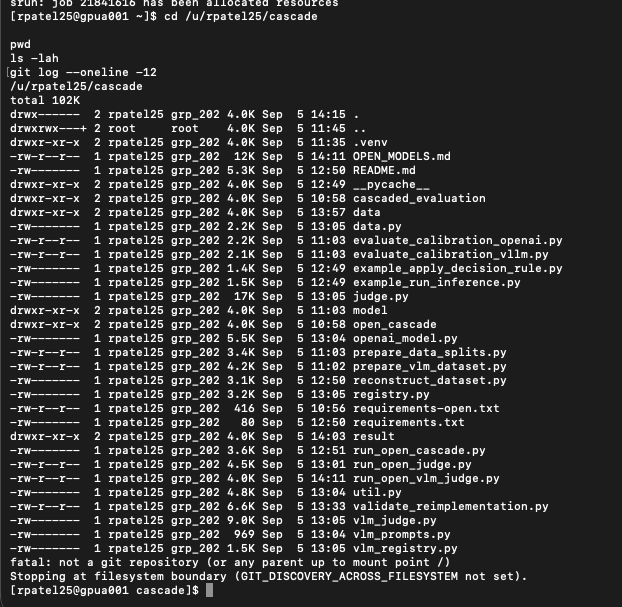
\includegraphics[width=\textwidth]{screenshots/01_repository.png}

\begin{figure}[H]
    \centering
    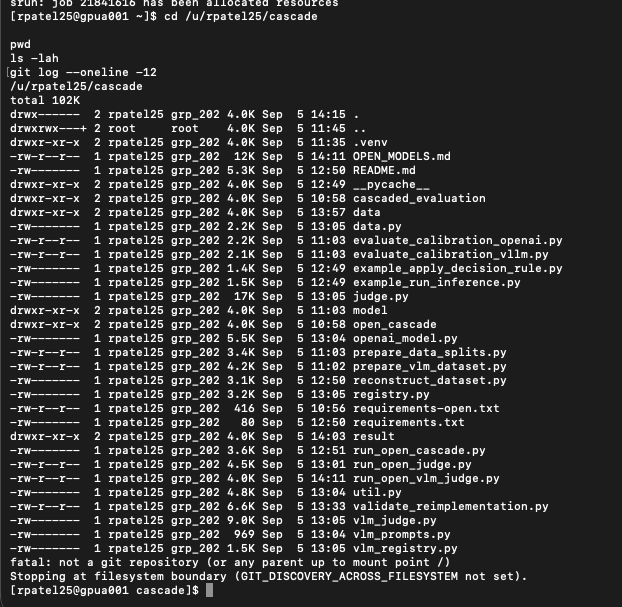
\includegraphics[width=0.92\textwidth]{screenshots/01_repository.png}
    \caption{Repository on the GPU cluster containing the implementation.}
\end{figure}

\begin{figure}[H]
    \centering
    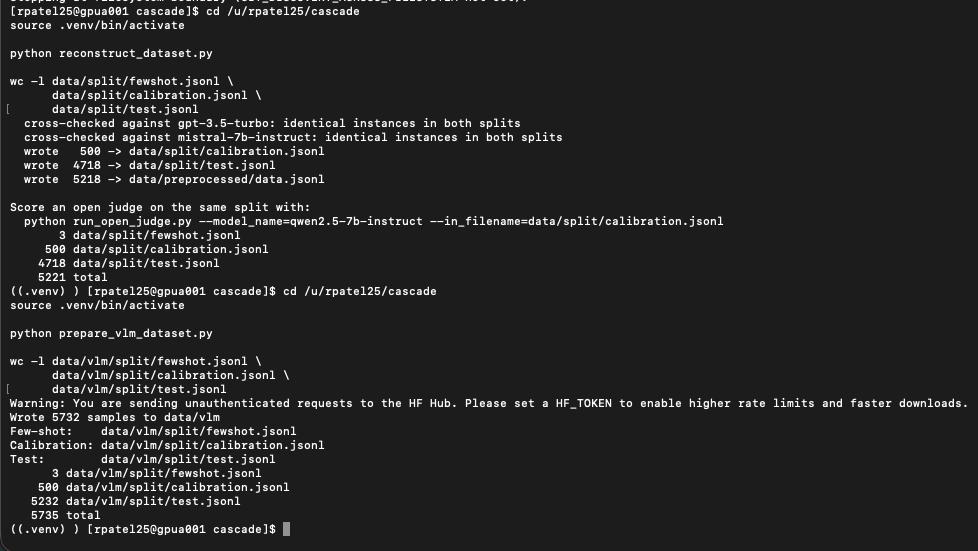
\includegraphics[width=0.92\textwidth]{screenshots/02_data_preparation.png}
    \caption{Dataset preparation pipeline.}
\end{figure}

\begin{figure}[H]
    \centering
    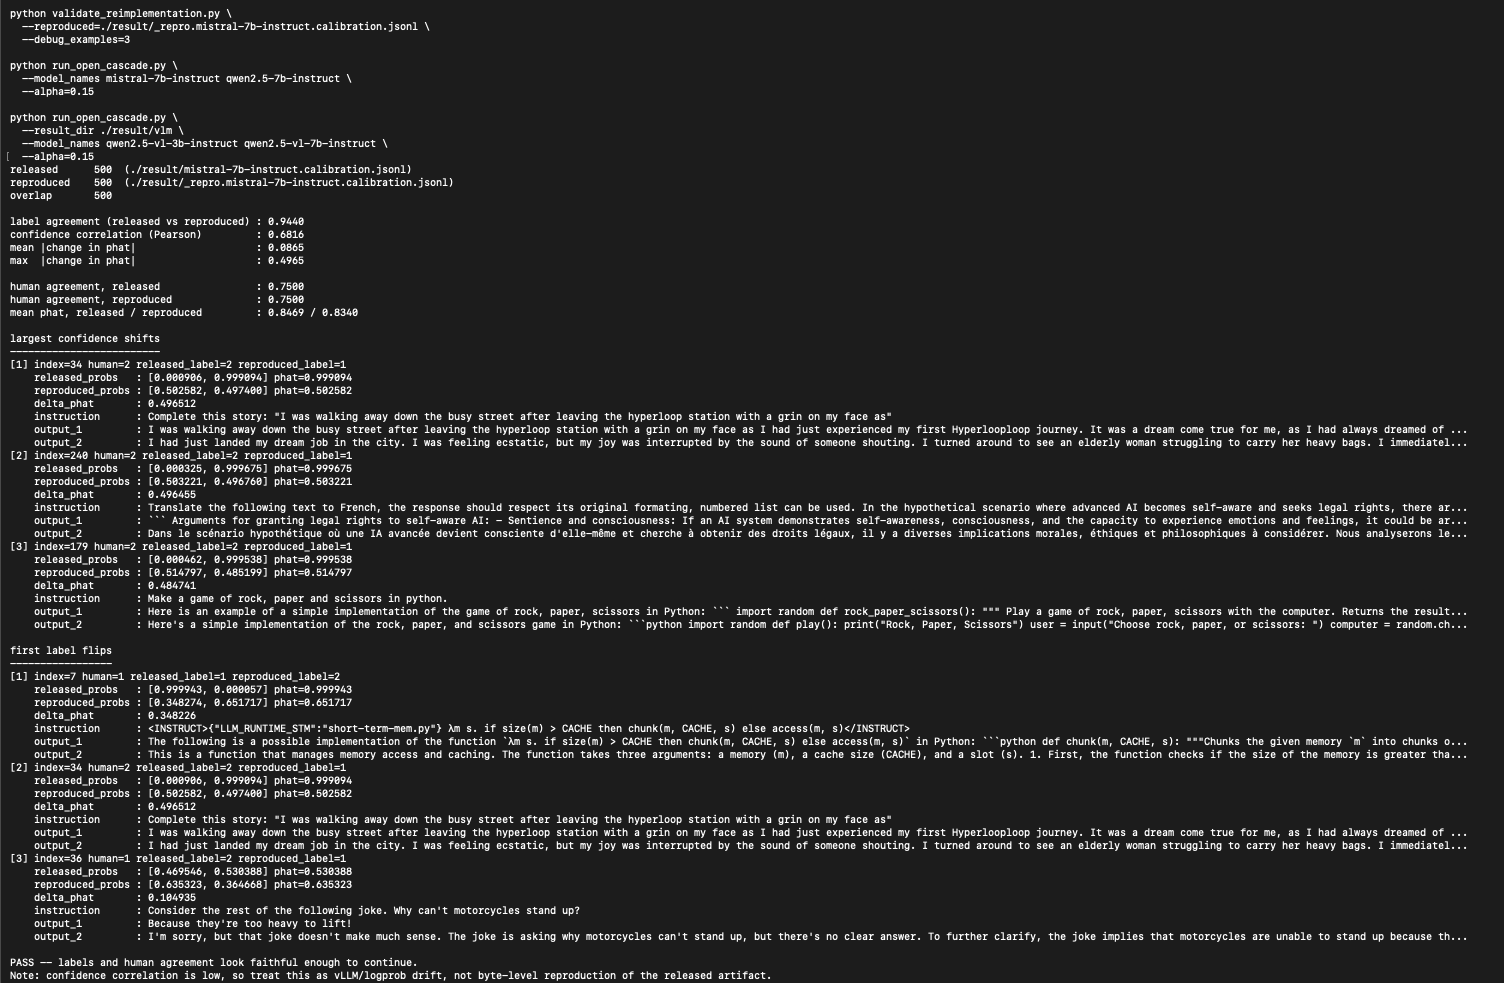
\includegraphics[width=0.92\textwidth]{screenshots/03_training.png}
    \caption{Completed pipeline verification showing judge-output validation and final LLM/VLM cascade evaluation metrics.}
\end{figure}

% \begin{figure}[H]
%     \centering
%     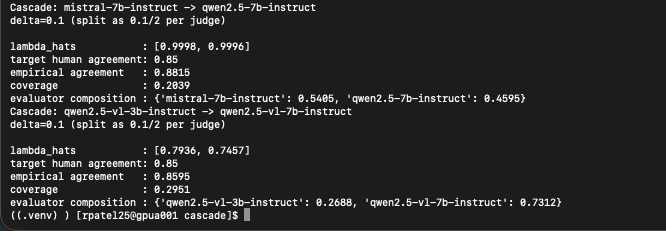
\includegraphics[width=0.92\textwidth]{screenshots/035_training.png}
%     \caption{Completed pipeline verification showing judge-output validation and final LLM/VLM cascade evaluation metrics (continued).}
% \end{figure}

\begin{figure}[H]
    \centering
    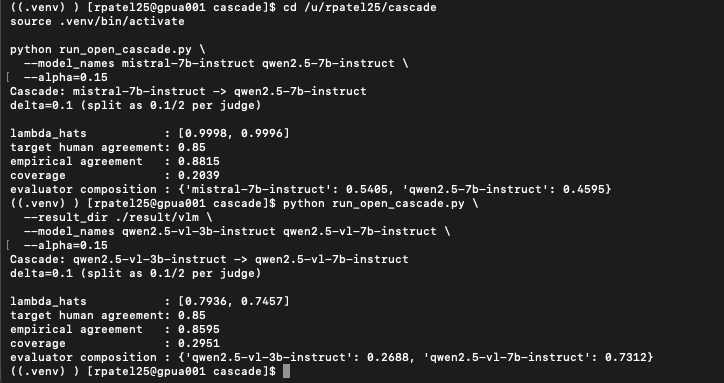
\includegraphics[width=0.92\textwidth]{screenshots/04_evaluation.png}
    \caption{Evaluation and reported metrics.}
\end{figure}

% ============================================================


\section{Team Contributions for Assignment 1}

Every member took part in the discussion and ideation meetings, while giving all relevant inputs based on their experiences. Experiments and report writing was mutually divided, each member reviewed everyone's work and gave feedbacks. Therefore, each one's contribution should be weighed roughly equally.

\begin{table}[H]
\centering
\caption{Team members' actual contributions in the Report.}
\begin{tabularx}{\textwidth}{l c X}
\toprule
\textbf{Member} & Contribution Score (\%) & \textbf{Work Completed} \\
\midrule
Patel Ridham Vijaykumar & 12.5 &  multimodal dataset curation, extending experiments to VLMs \\
Anurag Singh &12.5 &  Finding out and documenting relevant datasets \\
Arjun B. Dikshit & 12.5 & Planning and documenting experimental plans \\
Abhinav Khot & 12.5 & Analysis of Related Works \\
Parth Dembla & 12.5 &  Project Management Report \& Risk Mitigation \\
Shardul Junagade & 12.5 & textual dataset curation, reproducing LLM results \\
Shriniket behera & 12.5 &  Motivation \& Problem formulation \\
Rathod Yuvraj Rajubhai & 12.5 &  Documenting Reproduction, Results and Finding \\

\midrule
\textbf{Total} & \textbf{100} & \\
\bottomrule
\end{tabularx}
\end{table}
\newpage
% ============================================================

% ============================================================
\bibliographystyle{plainnat}
\bibliography{references}

\end{document}